% Created by tikzDevice version 0.12.6 on 2024-03-12 19:53:25
% !TEX encoding = UTF-8 Unicode
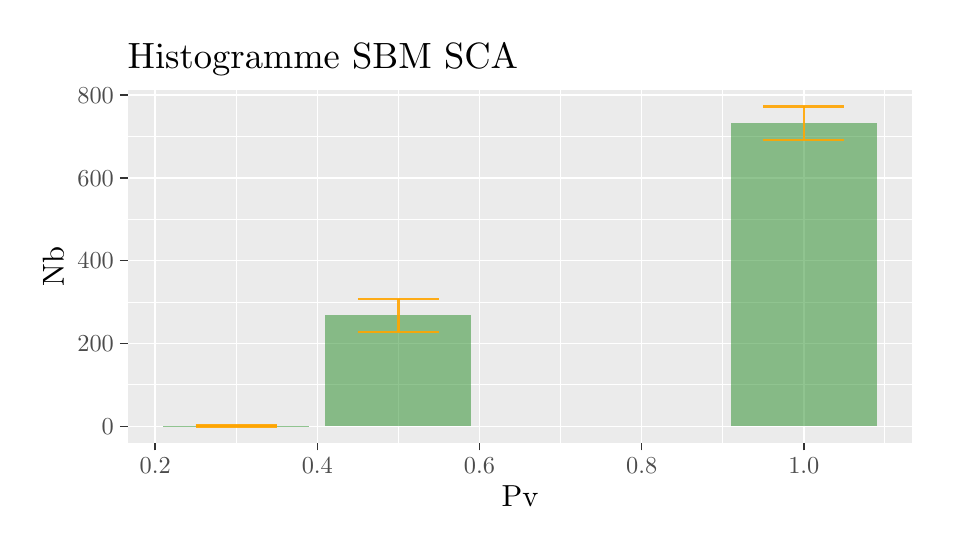
\begin{tikzpicture}[x=1pt,y=1pt]
\definecolor{fillColor}{RGB}{255,255,255}
\path[use as bounding box,fill=fillColor,fill opacity=0.00] (0,0) rectangle (325.21,180.67);
\begin{scope}
\path[clip] (  0.00,  0.00) rectangle (325.21,180.67);
\definecolor{drawColor}{RGB}{255,255,255}
\definecolor{fillColor}{RGB}{255,255,255}

\path[draw=drawColor,line width= 0.6pt,line join=round,line cap=round,fill=fillColor] (  0.00,  0.00) rectangle (325.21,180.68);
\end{scope}
\begin{scope}
\path[clip] ( 36.11, 30.69) rectangle (319.71,158.02);
\definecolor{fillColor}{gray}{0.92}

\path[fill=fillColor] ( 36.11, 30.69) rectangle (319.71,158.02);
\definecolor{drawColor}{RGB}{255,255,255}

\path[draw=drawColor,line width= 0.3pt,line join=round] ( 36.11, 51.59) --
	(319.71, 51.59);

\path[draw=drawColor,line width= 0.3pt,line join=round] ( 36.11, 81.53) --
	(319.71, 81.53);

\path[draw=drawColor,line width= 0.3pt,line join=round] ( 36.11,111.48) --
	(319.71,111.48);

\path[draw=drawColor,line width= 0.3pt,line join=round] ( 36.11,141.42) --
	(319.71,141.42);

\path[draw=drawColor,line width= 0.3pt,line join=round] ( 75.37, 30.69) --
	( 75.37,158.02);

\path[draw=drawColor,line width= 0.3pt,line join=round] (133.97, 30.69) --
	(133.97,158.02);

\path[draw=drawColor,line width= 0.3pt,line join=round] (192.56, 30.69) --
	(192.56,158.02);

\path[draw=drawColor,line width= 0.3pt,line join=round] (251.16, 30.69) --
	(251.16,158.02);

\path[draw=drawColor,line width= 0.3pt,line join=round] (309.75, 30.69) --
	(309.75,158.02);

\path[draw=drawColor,line width= 0.6pt,line join=round] ( 36.11, 36.61) --
	(319.71, 36.61);

\path[draw=drawColor,line width= 0.6pt,line join=round] ( 36.11, 66.56) --
	(319.71, 66.56);

\path[draw=drawColor,line width= 0.6pt,line join=round] ( 36.11, 96.51) --
	(319.71, 96.51);

\path[draw=drawColor,line width= 0.6pt,line join=round] ( 36.11,126.45) --
	(319.71,126.45);

\path[draw=drawColor,line width= 0.6pt,line join=round] ( 36.11,156.40) --
	(319.71,156.40);

\path[draw=drawColor,line width= 0.6pt,line join=round] ( 46.07, 30.69) --
	( 46.07,158.02);

\path[draw=drawColor,line width= 0.6pt,line join=round] (104.67, 30.69) --
	(104.67,158.02);

\path[draw=drawColor,line width= 0.6pt,line join=round] (163.26, 30.69) --
	(163.26,158.02);

\path[draw=drawColor,line width= 0.6pt,line join=round] (221.86, 30.69) --
	(221.86,158.02);

\path[draw=drawColor,line width= 0.6pt,line join=round] (280.46, 30.69) --
	(280.46,158.02);
\definecolor{fillColor}{RGB}{34,139,34}

\path[fill=fillColor,fill opacity=0.50] ( 49.00, 36.61) rectangle (101.74, 36.68);

\path[fill=fillColor,fill opacity=0.50] (107.60, 36.61) rectangle (160.33, 76.73);

\path[fill=fillColor,fill opacity=0.50] (254.09, 36.61) rectangle (306.82,146.16);
\definecolor{drawColor}{RGB}{255,165,0}

\path[draw=drawColor,draw opacity=0.90,line width= 0.9pt,line join=round] ( 60.72, 36.88) --
	( 90.02, 36.88);

\path[draw=drawColor,draw opacity=0.90,line width= 0.9pt,line join=round] ( 75.37, 36.88) --
	( 75.37, 36.47);

\path[draw=drawColor,draw opacity=0.90,line width= 0.9pt,line join=round] ( 60.72, 36.47) --
	( 90.02, 36.47);

\path[draw=drawColor,draw opacity=0.90,line width= 0.9pt,line join=round] (119.32, 82.71) --
	(148.62, 82.71);

\path[draw=drawColor,draw opacity=0.90,line width= 0.9pt,line join=round] (133.97, 82.71) --
	(133.97, 70.76);

\path[draw=drawColor,draw opacity=0.90,line width= 0.9pt,line join=round] (119.32, 70.76) --
	(148.62, 70.76);

\path[draw=drawColor,draw opacity=0.90,line width= 0.9pt,line join=round] (265.81,152.23) --
	(295.10,152.23);

\path[draw=drawColor,draw opacity=0.90,line width= 0.9pt,line join=round] (280.46,152.23) --
	(280.46,140.08);

\path[draw=drawColor,draw opacity=0.90,line width= 0.9pt,line join=round] (265.81,140.08) --
	(295.10,140.08);
\end{scope}
\begin{scope}
\path[clip] (  0.00,  0.00) rectangle (325.21,180.67);
\definecolor{drawColor}{gray}{0.30}

\node[text=drawColor,anchor=base east,inner sep=0pt, outer sep=0pt, scale=  0.88] at ( 31.16, 33.58) {0};

\node[text=drawColor,anchor=base east,inner sep=0pt, outer sep=0pt, scale=  0.88] at ( 31.16, 63.53) {200};

\node[text=drawColor,anchor=base east,inner sep=0pt, outer sep=0pt, scale=  0.88] at ( 31.16, 93.47) {400};

\node[text=drawColor,anchor=base east,inner sep=0pt, outer sep=0pt, scale=  0.88] at ( 31.16,123.42) {600};

\node[text=drawColor,anchor=base east,inner sep=0pt, outer sep=0pt, scale=  0.88] at ( 31.16,153.37) {800};
\end{scope}
\begin{scope}
\path[clip] (  0.00,  0.00) rectangle (325.21,180.67);
\definecolor{drawColor}{gray}{0.20}

\path[draw=drawColor,line width= 0.6pt,line join=round] ( 33.36, 36.61) --
	( 36.11, 36.61);

\path[draw=drawColor,line width= 0.6pt,line join=round] ( 33.36, 66.56) --
	( 36.11, 66.56);

\path[draw=drawColor,line width= 0.6pt,line join=round] ( 33.36, 96.51) --
	( 36.11, 96.51);

\path[draw=drawColor,line width= 0.6pt,line join=round] ( 33.36,126.45) --
	( 36.11,126.45);

\path[draw=drawColor,line width= 0.6pt,line join=round] ( 33.36,156.40) --
	( 36.11,156.40);
\end{scope}
\begin{scope}
\path[clip] (  0.00,  0.00) rectangle (325.21,180.67);
\definecolor{drawColor}{gray}{0.20}

\path[draw=drawColor,line width= 0.6pt,line join=round] ( 46.07, 27.94) --
	( 46.07, 30.69);

\path[draw=drawColor,line width= 0.6pt,line join=round] (104.67, 27.94) --
	(104.67, 30.69);

\path[draw=drawColor,line width= 0.6pt,line join=round] (163.26, 27.94) --
	(163.26, 30.69);

\path[draw=drawColor,line width= 0.6pt,line join=round] (221.86, 27.94) --
	(221.86, 30.69);

\path[draw=drawColor,line width= 0.6pt,line join=round] (280.46, 27.94) --
	(280.46, 30.69);
\end{scope}
\begin{scope}
\path[clip] (  0.00,  0.00) rectangle (325.21,180.67);
\definecolor{drawColor}{gray}{0.30}

\node[text=drawColor,anchor=base,inner sep=0pt, outer sep=0pt, scale=  0.88] at ( 46.07, 19.68) {0.2};

\node[text=drawColor,anchor=base,inner sep=0pt, outer sep=0pt, scale=  0.88] at (104.67, 19.68) {0.4};

\node[text=drawColor,anchor=base,inner sep=0pt, outer sep=0pt, scale=  0.88] at (163.26, 19.68) {0.6};

\node[text=drawColor,anchor=base,inner sep=0pt, outer sep=0pt, scale=  0.88] at (221.86, 19.68) {0.8};

\node[text=drawColor,anchor=base,inner sep=0pt, outer sep=0pt, scale=  0.88] at (280.46, 19.68) {1.0};
\end{scope}
\begin{scope}
\path[clip] (  0.00,  0.00) rectangle (325.21,180.67);
\definecolor{drawColor}{RGB}{0,0,0}

\node[text=drawColor,anchor=base,inner sep=0pt, outer sep=0pt, scale=  1.10] at (177.91,  7.64) {Pv};
\end{scope}
\begin{scope}
\path[clip] (  0.00,  0.00) rectangle (325.21,180.67);
\definecolor{drawColor}{RGB}{0,0,0}

\node[text=drawColor,rotate= 90.00,anchor=base,inner sep=0pt, outer sep=0pt, scale=  1.10] at ( 13.08, 94.35) {Nb};
\end{scope}
\begin{scope}
\path[clip] (  0.00,  0.00) rectangle (325.21,180.67);
\definecolor{drawColor}{RGB}{0,0,0}

\node[text=drawColor,anchor=base west,inner sep=0pt, outer sep=0pt, scale=  1.32] at ( 36.11,166.08) {Histogramme SBM SCA};
\end{scope}
\end{tikzpicture}
